\chapter{Bearings Faults Diagnostic using Neural Networks}

\chapterintrobox{Vibration condition monitoring are vital for many industrial systems, vibration data contains very useful information about health state of the equipment. Nevertheless, gaining insights from vibration signals in real-world applications turns out to be a complex—and in many times, unfruitful—process. This is mainly due to the complexity of the problem. This chapter demonstrates image processing based approach for bearings faults diagnostics using convolutional neural networks.}

\section{Case Western Reserve University Bearings Data}

\begin{wrapfigure}{r}{0.5\textwidth}
    \centering
	\begin{tikzpicture}
	\node (outer) at (3.5,1.2) {\makecell{\small Outer\\Race}};
	\node (inner) at (3.5,0) {\makecell{\small Inner\\Race}};
	\node (ball) at (3.5,-1.2) {\makecell{\small Ball\\(in cage)}};
	
	\node (outer2) at (1.3,1.2) {};
	\node (inner2) at (.3,0) {};
	\node (ball2) at (-.5,-1.2) {};

	\node[inner sep=0] (image) at (0,0) {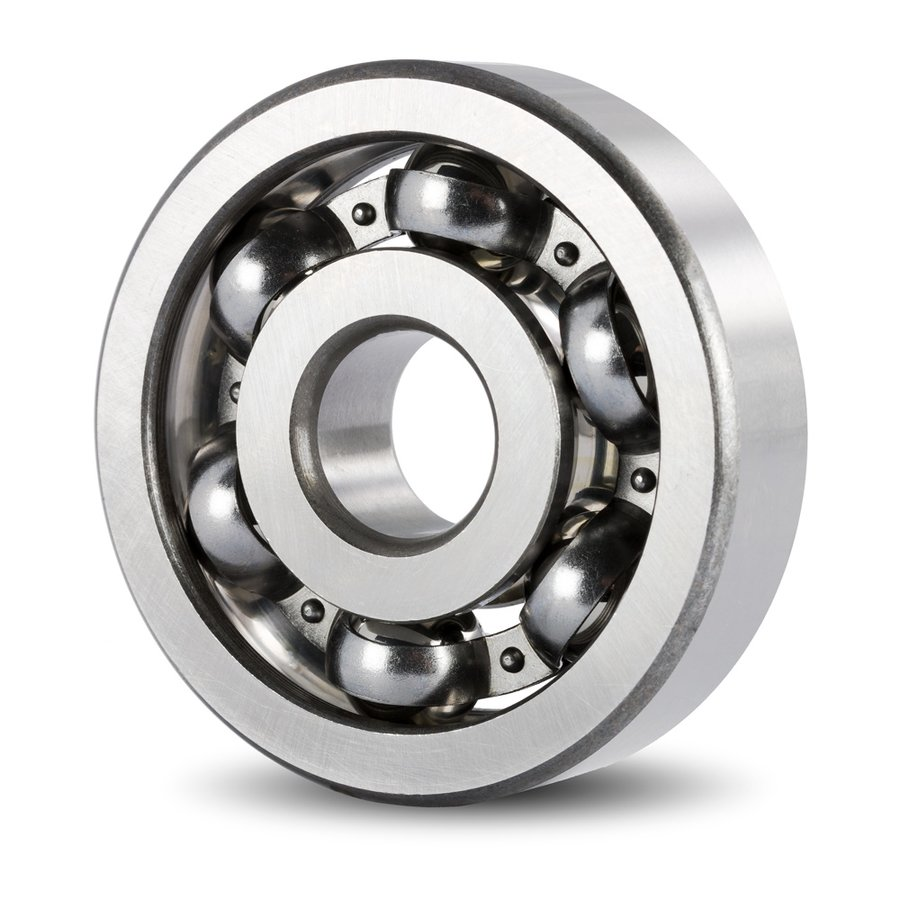
\includegraphics[width=0.35\textwidth]{figures/skf.jpg}};

	\draw [|->,  thick, red] (outer.west) -- (outer2);
	\draw [|->,  thick, red] (ball) -- (ball2);
	\draw [|->,  thick, red] (inner) -- (inner2);
\end{tikzpicture}
	\caption{Bearing's components}
    \label{figure:skf-bearing-components}    
\end{wrapfigure}
\vspace{-1em}

The dataset used in this chapter is bearings vibration dataset provided by Case Western Reserve University (CWRU). The bearings used in the test are SKF ball bearings. Figure \ref{figure:skf-bearing-components} shows the different components of a standard ball bearing.The test was conducted where the bearings support the shaft of a 2hp motor at different loading conditions. 

The test bearings have single point faults which were introduced using electro-discharge matching with fault diameters of 0.18mm, 0.36mm, 0.53mm, 0.71mm and 1.02mm. These faults were introduced in the bearing's ball, inner and outer raceways. SKF bearings were used for the 0.18mm, 0.36mm and 0.53mm faults, and NTN equivalent were used for the 0.71mm and 1.02mm faults. Table \ref{table:cwru-bearings-specification} contains the used SKF bearings' model dimensions and the corresponding frequencies (as multiples of RPM) associated with with different faults types.

\begin{table}[H]
	\centering
	\begin{tabu}{cc|[1.5pt]cc}
		\tabucline[1.5pt]{-} 
		Dimension		&	Size (mm)	&	Defect 			& Frequency ($\times$RPM Hz)	\\
		\hline
		Inner Diameter	&	25.00		& Inner Ring 		& 5.4152\\
		Outside Diameter&	52.00		& Outer Ring 		& 3.5848 \\
		Thickness 		&	15.00		& Cage Train		& 0.3983 \\
		Pitch Diameter	&	08.03		& Rolling Element	& 4.7135\\
		\tabucline[1.5pt]{-} 
	\end{tabu}
	\caption{CWRU bearings dimensions and faults frequencies}
	\label{table:cwru-bearings-specification}
\end{table}

\section{Generating data from raw vibration signals}
Raw vibration data can't be used directly as an input to a neural network. This chapter uses the approach proposed in \cite{Wen2018} to convert raw vibration data into images. Figure \ref{fig:cw_bearings_data_generation} shows data generation principal where 1-dimensional vibration signals are converted into 2-dimensional arrays (images) by reshaping chunks of length 4096 into matrices of 64$\times$64.

\begin{figure}[h]
	\centering
	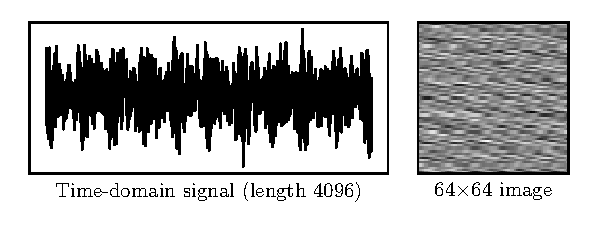
\includegraphics{figures/cw_bearings_data_generation.pdf}
	\caption{Data generation by converting the signal into 64$\times$64 images}
	\label{fig:cw_bearings_data_generation}
\end{figure}

As mentioned before, several tests have been conducted with different types of bearings faults (i.e. ball, inner and outer raceways faults) with different fault diameters. Signals from the different tests are transformed into images to serve as an input for a convolutional neural network which will be trained to classify the different signals into the corresponding fault types and their diameters. Signals are distributed across 10 classes: three different fault types and for each fault type there are three different fault diameters, plus a normal baseline signal that belongs to healthy bearing. Figure \ref{fig:bearings_faults_samples} shows some samples of the transformed signals of the different nine fault types/diameters: 

\begin{figure}[h]
    \centering
	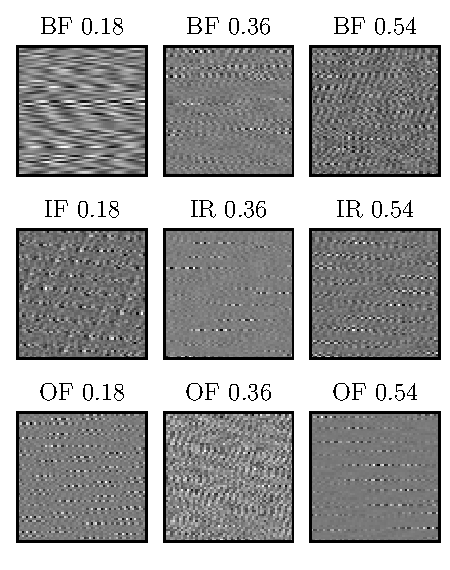
\includegraphics{figures/cw_bearings_faults_samples.pdf}
    \caption{Converted signals of different faults types}
    \label{fig:bearings_faults_samples}
\end{figure}

Signals of the different fault types have varying lengths which results in a different number of synthesized images per fault type. Number of images per class is given by equation \ref{equation:labels-per-class}:

\begin{equation}
	N=floor \left(\frac{\text{signal length}}{64\times64}\right)
	\label{equation:labels-per-class}
\end{equation}

Number of images corresponding to each class is showin in Figure \ref{fig:bearings_faults_samples_count}:

\begin{figure}[h]
    \centering
	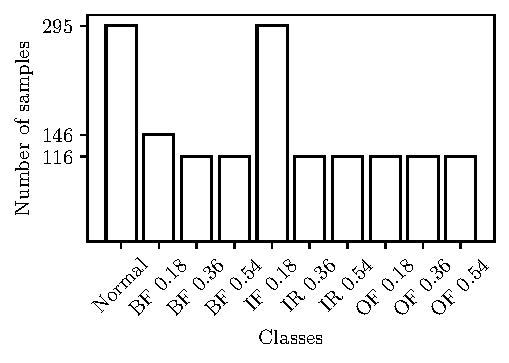
\includegraphics{figures/cw_bearings_faults_count.pdf}
    \caption{Converted signals of different faults types}
	\label{fig:bearings_faults_samples_count}
\end{figure}
\begin{comment}
\begin{table}[h]
	\centering
	\begin{tabu}{lc}
		\tabucline[1.5pt]{-} 
	   Class 					&	Samples count	\\
	   \hline 
	   Normal bearing 			&	295				\\
	   Roller element 0.18mm 	&	146				\\
	   Roller element 0.36mm 	&	116				\\
	   Roller element 0.54mm	&	116				\\
	   Inner race 0.18mm		&	295				\\
	   Inner race 0.36mm		&	116				\\
	   Inner race 0.54mm		&	116				\\
	   Outer race 0.18mm		&	116				\\
	   Outer race 0.36mm		&	116				\\
	   Outer race 0.54mm		&	116				\\
   \tabucline[1.5pt]{-}
   \end{tabu}
   \caption{}
   \label{table:cw-classes-count}
\end{table}
\end{comment}

\section{Bearings faults diagnostic using neural networks}
After generating data by converting raw vibration signals into images, these images serve as an input for a convolutional neural network.

\subsection{Network architecture}
\acrlong{cnn} (\acrshort{cnn}) describes a type of neural networks that is suitable for image processing. This section presents the use of \acrshort{cnn} to classify bearings vibration signals that have been transformed into images into the corresponding fault types. CNN were described in details in section \ref{section:cnn}.

To perform this classification task, a \acrshort{cnn} architecture is used, the network consists of three convolutional layers with max-pooling layers in between, followed by three fully-connected layers. All the details of this architecture from are mentioned in Table \ref{table:bearings-faults-cnn-classifier-architecture}.


\begin{comment}
\begin{figure}[h]
	\centering
		\begin{tikzpicture}
	[blend group = soft light]
	
	\tikzstyle{input} = [rectangle, minimum width = 8em, minimum height = 3em, rounded corners=4pt, thick, draw ]
	
	\tikzstyle{convolution} = [rectangle, minimum width = 8em, minimum height = 3em, rounded corners=4pt, thick, draw ]
	
	\tikzstyle{maxpooling} = [rectangle, minimum width = 8em, minimum height = 3em, rounded corners=4pt, thick, draw ]
	
	\tikzstyle{flatten} = [rectangle,minimum width = 8em, minimum height = 3em, rounded corners=4pt, thick, draw  ]
	
	\tikzstyle{fc} = [rectangle, minimum width = 8em, minimum height = 3em, rounded corners=4pt, thick, draw ]
	
		\node[input] (input-node) {\makecell[c]{Input\\ \small{64$\times$64}}};
		
		\node[convolution, below = 1em of input-node](conv1) {\makecell[c]{
				Convolution\\
				\footnotesize{3$\times$3, 32 filters}
			}};
		
		\node[maxpooling, below = 1em of conv1](maxpool1) {\makecell[c]{
				MaxPooling\\
				\footnotesize{2$\times$2}
		}};
	
	\node[convolution, below = 1em of maxpool1](conv2) {\makecell[c]{
			Convolution\\
			\footnotesize{3$\times$3, 64 filters}
	}};

\node[maxpooling, below = 1em of conv2](maxpool2) {\makecell[c]{
		MaxPooling\\
		\footnotesize{2$\times$2}
}};

\node[convolution, below = 1em of maxpool2](conv3) {\makecell[c]{
		Convolution\\
		\footnotesize{3$\times$3, 128 filters}
}};

\node[maxpooling, below = 1em of conv3](maxpool3) {\makecell[c]{
		MaxPooling\\
		\footnotesize{2$\times$2}
}};

\node[fc, below = 1em of maxpool3](flatten) {Flatten};

\node[convolution, below = 1em of flatten](fc1) {\makecell[c]{
		Fully-connected\\
		\footnotesize{128 neurons, ReLU}
}};

\node[fc, below = 1em of fc1](fc2) {\makecell[c]{
		Fully-connected\\
		\footnotesize{64 neurons, ReLU}
}};

\node[fc, below = 1em of fc2](fc3) {\makecell[c]{
		Fully-connected\\
		\footnotesize{10 neurons, Softmax}
}};

\draw[->] (input-node) -- (conv1);
\draw[->] (conv1) -- (maxpool1);
\draw[->] (maxpool1) -- (conv2);
\draw[->] (conv2) -- (maxpool2);
\draw[->] (maxpool2) -- (conv3);
\draw[->] (conv3) -- (maxpool3);
\draw[->] (maxpool3) -- (flatten);
\draw[->] (flatten) -- (fc1);
\draw[->] (fc1) -- (fc2);
\draw[->] (fc2) -- (fc3);
\end{tikzpicture}
	
	\caption{}
	\label{}
\end{figure}
\end{comment}

\begin{table}[h]
    \centering
    \begin{tabu}{lll}
		\tabucline[1.5pt]{-}
		\textbf{Layer (type)}   & \textbf{Output shape} &   \textbf{Param \#} \\
		\tabucline[1pt]{-}
		Conv1 (Conv2D) 			&   (None, 1, 64 ,32)   &   18464   \\
		MaxPool1 (MaxPool2D) 	&   (None, 1, 32, 32)   &   0       \\
		Conv2 (Conv2D)			&   (None, 1, 32, 64)   &   18496   \\
		MaxPool2 (MaxPooling2D) &   (None, 1, 16, 64)   &   0       \\
		Conv3 (Conv2D)          &   (None, 1, 16, 128)  &   73856   \\
		MaxPool3 (MaxPooling2D) &   (None, 1, 8, 128)   &   0       \\       
		Flatten1 (Flatten)      &   (None, 1024)        &   0       \\     
		Dense1 (Dense)          &   (None, 128)         &   131200  \\   
		Dense2 (Dense)          &   (None, 64)          &   8256    \\     
		Dense3 (Dense)          &   (None, 10)          &   650     \\
		\tabucline[1pt]{-}
		Total params: 250,922       &                   &           \\
		Trainable params: 250,922   &                   &           \\
		Non-trainable params: 0     &                   &           \\
	\tabucline[1.5pt]{-}
    \end{tabu}
    \caption{CNN architecture}
    \label{table:bearings-faults-cnn-classifier-architecture}
\end{table}

The network is developed using Python and Keras framework \cite{chollet2015keras}.

\subsection{Training process}
The dataset contains in total 1548 samples, 20\% is used as a test set while the remaining 80\% is the training set. From the train set, 15\% is used as a validation split during the training process. The network was trained for 30 epochs and a batch size of 32.
Figure \ref{fig:bearings_faults_classification_training} shows the evolution of the accuracy (\%) and loss (categorical cross-entropy) as a function of training epochs. The network converges around 10th epoch with minor increase in accuracy and decrease in loss afterwards. 

\begin{figure}[h]
    \centering
    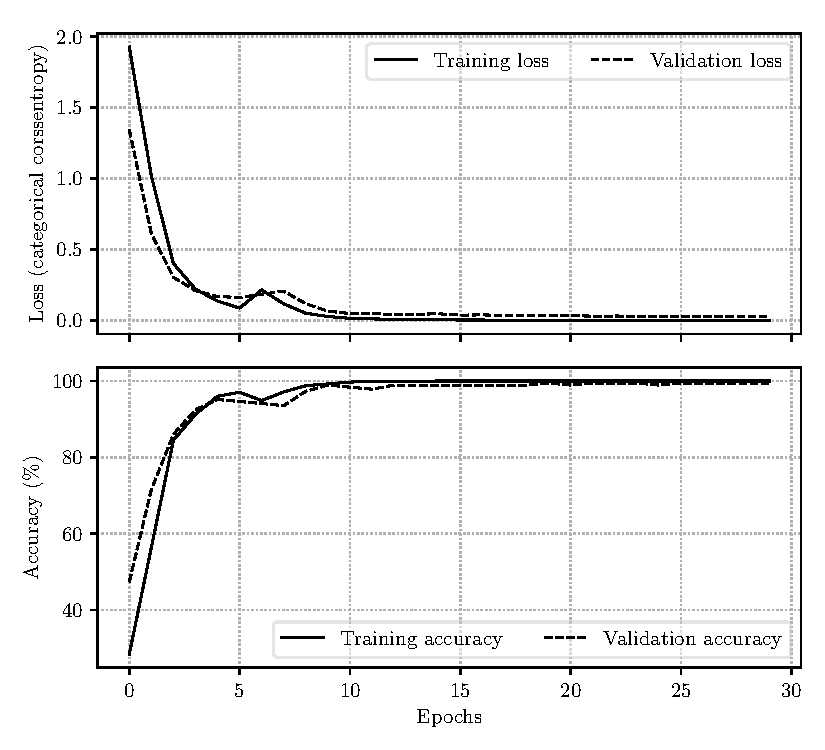
\includegraphics{figures/cw_bearings_faults_classification_training.pdf}
    \caption{Classifier training}
    \label{fig:bearings_faults_classification_training}
\end{figure}

\subsection{Network results discussion}
The model achieves perfect 100\% accuracy on training set and a close accuracy on validation set. After training the model is evaluated on the test set and achieves a near perfect accuracy of 98.72\% accuracy. Train, validation and test loss and accuracy are summarized in Table \ref{table:cw-cnn-results}.

\begin{table}[H]
	\centering
	\begin{tabu}{lcc}
		\tabucline[1.5pt]{2-3} 
						&	\textbf{Loss}	&	\textbf{Accuracy}	\\
	   \tabucline[1pt]{-}
		Train set 		&	0.0003			&	100.00\%				\\
		Validation set 	&	0.0269 			&	99.46\%					\\
		Test set		&	0.0586 			&	98.71\%					\\
   \tabucline[1.5pt]{-}
   \end{tabu}
   \caption{CNN training results}
   \label{table:cw-cnn-results}
\end{table}

To further understand the model's results, confusion matrix is constructed. The confusion matrix (Figure \ref{fig:bearings_faults_classification_confusion_matrix}) shows the results of model predictions on the test set where y-axis shows the actual (real) labels in the test set and x-axis the model predictions. Diagnoal of confusion matrix is where actual labels intersect with model's predicted labels for each sample and it is apparent that the model achieves near-perfect classification.

\begin{figure}[h]
    \centering
    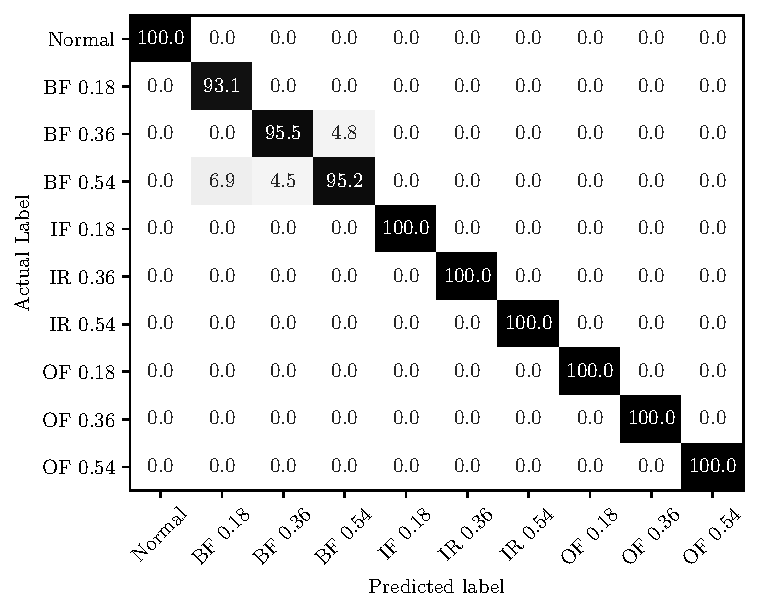
\includegraphics{figures/cw_bearings_faults_classification.pdf}
    \caption{Confusion matrix of bearings faults classification using CNN}
    \label{fig:bearings_faults_classification_confusion_matrix}
\end{figure}

\section{Conclusion}
This chapter adopted a data generation approach from literature that converts vibration signals into images. Vibration signals used here corresponds to bearings with different types of faults and fault diameters. After converting raw signals into images, a \acrshort{cnn} is used to classify transformed signals (i.e. images) into their corresponding faults types and diameters. The model achieves near-perfect classification accuracy on the test set.

